\documentclass[supercite]{Experimental_Report}

\title{~~~~~~数据结构实验~~~~~~}
\author{严浩洋}
%\coauthor{张三、李四}
\school{计算机科学与技术学院}
\classnum{CS2209}
\stunum{U202215650}
%\costunum{U202115631、U202115631}
\instructor{李剑军} % 该系列实验报告模板有华科大计院教师陈加忠制作
\date{2022年6月1日}

\usepackage{algorithm, multirow}
\usepackage{algpseudocode}
\usepackage{amsmath}
\usepackage{amsthm}
\usepackage{framed}
\usepackage{mathtools}
\usepackage{fontspec}
\usepackage{subcaption}
\usepackage{xltxtra} %提供了针对XeTeX的改进并且加入了XeTeX的LOGO, 自动调用xunicode宏包(提供Unicode字符宏)
\usepackage{bm}
\usepackage{tikz}
\usepackage{tikzscale}
\usepackage{pgfplots}
\usepackage{textcomp}
\usepackage{listings}
\usepackage{xcolor}
\lstset{
	basicstyle=\tiny,
    numbers=left, 
    %numberstyle= \tiny, 
    keywordstyle= \color{ blue!70},
    commentstyle= \color{red!50!green!50!blue!50}, 
    %frame=shadowbox, % 阴影效果
    rulesepcolor= \color{ red!20!green!20!blue!20} ,
	stringstyle=\ttfamily,
	breaklines=true,
	escapebegin=\begin{CJK*}{GBK}{hei},escapeend=\end{CJK*},
	escapeinside=``, % 英文分号中可写入中文
    %xleftmargin=2em,xrightmargin=2em, aboveskip=1em,
    %framexleftmargin=2em
}
%\usepackage{enumerate}

\pgfplotsset{compat=1.16}

\newcommand{\cfig}[3]{
  \begin{figure}[htb]
    \centering
    \includegraphics[width=#2\textwidth]{images/#1.tikz}
    \caption{#3}
    \label{fig:#1}
  \end{figure}
}

\newcommand{\sfig}[3]{
  \begin{subfigure}[b]{#2\textwidth}
    \includegraphics[width=\textwidth]{images/#1.tikz}
    \caption{#3}
    \label{fig:#1}
  \end{subfigure}
}

\newcommand{\xfig}[3]{
  \begin{figure}[htb]
    \centering
    #3
    \caption{#2}
    \label{fig:#1}
  \end{figure}
}

\newcommand{\rfig}[1]{\autoref{fig:#1}}
\newcommand{\ralg}[1]{\autoref{alg:#1}}
\newcommand{\rthm}[1]{\autoref{thm:#1}}
\newcommand{\rlem}[1]{\autoref{lem:#1}}
\newcommand{\reqn}[1]{\autoref{eqn:#1}}
\newcommand{\rtbl}[1]{\autoref{tbl:#1}}

\algnewcommand\Null{\textsc{null }}
\algnewcommand\algorithmicinput{\textbf{Input:}}
\algnewcommand\Input{\item[\algorithmicinput]}
\algnewcommand\algorithmicoutput{\textbf{Output:}}
\algnewcommand\Output{\item[\algorithmicoutput]}
\algnewcommand\algorithmicbreak{\textbf{break}}
\algnewcommand\Break{\algorithmicbreak}
\algnewcommand\algorithmiccontinue{\textbf{continue}}
\algnewcommand\Continue{\algorithmiccontinue}
\algnewcommand{\LeftCom}[1]{\State $\triangleright$ #1}

\newtheorem{thm}{定理}[section]
\newtheorem{lem}{引理}[section]

\colorlet{shadecolor}{black!15}

\theoremstyle{definition}
\newtheorem{alg}{算法}[section]

\def\thmautorefname~#1\null{定理~#1~\null}
\def\lemautorefname~#1\null{引理~#1~\null}
\def\algautorefname~#1\null{算法~#1~\null}

\begin{document}

\maketitle

\clearpage

\pagenumbering{Roman}

\tableofcontents[level=2]

\clearpage

\pagenumbering{arabic}

\section{基于顺序存储结构的线性表实现}

%图\ref{fig1-1}只是网页整体框架举例,它是用visio画的,然后再在visio里通过文件-打印,如图\ref{fig1-2}所示打印成pdf文件,然后再用pdf阅览器的工具,如图\ref{fig1-3}所示,做适当的裁剪。画图说明网页的整体框架,进行简要的文字描述等。画图说明网页的整体框架,进行简要的文字描述等。画图说明网页的整体框架,进行简要的文字描述等。画图说明网页的整体框架,进行简要的文字描述等。画图说明网页的整体框架,进行简要的文字描述等。画图说明网页的整体框架,进行简要的文字描述等。画图说明网页的整体框架,进行简要的文字描述等。

%请注意,当正文中出现1) 2) 3)罗列时,请必须用enumerate环境,具体如下!
% \begin{enumerate}
% \renewcommand{\labelenumi}{\theenumi)}
% 	\item C++
% 	\item Java
% 	\item HTML
% \end{enumerate}
%画图说明网页的整体框架,进行简要的文字描述等。画图说明网页的整体框架,进行简要的文字描述等。画图说明网页的整体框架,进行简要的文字描述等。画图说明网页的整体框架,进行简要的文字描述等。画图说明网页的整体框架,进行简要的文字描述等。画图说明网页的整体框架,进行简要的文字描述等。画图说明网页的整体框架,进行简要的文字描述等。
\subsection{问题描述}
实验要求构造顺序表,并创建一个菜单来实现功能的演示。功能包括\textbf{基础的}创建销毁与增删改查等操作,以及\textbf{进阶的}文件存取、多线性表管理与求最大子数组和等实用功能。

\subsubsection{功能实现}

具体实现的功能如下:
\begin{enumerate}
	\item 基础功能
	\begin{enumerate}
		\item 初始化表
		\item 销毁表
		\item 清空表
		\item 判定空表
		\item 求表长
		\item 获取元素
		\item 查找元素
		\item 获得前驱
		\item 获得后继
		\item 插入元素
		\item 删除元素
		\item 遍历表
	\end{enumerate}
	\item 进阶功能

	\color{black}\begin{enumerate}
		\item 最大连续子数组和
		\item 和为K的子数组
		\item 顺序表排序
		\item 文件形式存取线性表
		\item 多线性表管理
	\end{enumerate}
\end{enumerate}

\subsubsection{实验目的}

\begin{enumerate}
	\item 加强对线性表与顺序存储结构的理解和使用,掌握实现线性表基础功能的方法。
	\item 通过对顺序存储结构的实现,了解顺序表逻辑结构与物理结构的关系。
	\item 会运用线性表实现常用的功能,并解决常见的问题。
\end{enumerate}
%说明此实验要解决的基本问题。大力出奇迹!!!参考文献无法显示怎么办?陈老师正在想办法解决\cite{STR2021Neurocom, AVS2021Neurocom}!我是参考文献。我是第二小节\cite{Mehrabian1974An}。我是第二小节\cite{Rezaei2014CVPR}。我是第二小节\cite{Ramnath2008IJCV}。

\subsection{系统设计}
%包括整体系统结构设计和数据结构设计等。先在文件夹里的bib文件里添加新的参考文献,给每篇参考文献取一个索引的名字,然后再引用比如\cite{STR2021Neurocom}\cite{AVS2021Neurocom, Rezaei2014CVPR}。请注意书籍、期刊论文、专利等bib条目的格式是不一样的。画图说明网页的整体框架,进行简要的文字描述等。画图说明网页的整体框架,进行简要的文字描述等。画图说明网页的整体框架,进行简要的文字描述等。画图说明网页的整体框架,进行简要的文字描述等。画图说明网页的整体框架,进行简要的文字描述等。画图说明网页的整体框架,进行简要的文字描述等。画图说明网页的整体框架,进行简要的文字描述等。
\subsubsection{系统总体设计}
本系统在初始条件下提供一个顺序存储结构的线性表,用户可自行添加新的线性表或删除原有的线性表,总表数不超过十个。每个线性表\textbf{相互独立},均可独立实现所有的功能。系统所能实现的功能包括基础功能和进阶功能两部分,已在上一节中列出。

系统利用一个简易菜单以供用户选择需要的功能。通过\textbf{清屏函数}等操作,并用\textbf{system}相关函数调整窗口大小,可以使菜单选项始终位于界面上方,方便用户选择。

主函数中主要包括相关变量的定义以及菜单的实现,利用\textbf{switch分支结构}以实现功能的选择,并将特定的功能分别封装于不同的函数中。在主函数中只需调用相应函数即可。
\subsubsection{数据结构设计}
本实验以顺序存储结构线性表为主体,但定义了新的结构:Lists,用于多线性表管理。

Lists包含两部分:Lists的长度和最多可存储十个SqList的数组。前者用于表示管理线性表的个数,后者用于存储线性表。

\newpage

\subsection{系统实现}
%主要说明各个主要函数的实现思想,复杂函数可辅助流程图进行说明,函数和系统实现的源代码放在附录中。画图说明网页的整体框架,进行简要的文字描述等。画图说明网页的整体框架,进行简要的文字描述等。画图说明网页的整体框架,进行简要的文字描述等。画图说明网页的整体框架,进行简要的文字描述等。画图说明网页的整体框架,进行简要的文字描述等。画图说明网页的整体框架,进行简要的文字描述等。画图说明网页的整体框架,进行简要的文字描述等。
\subsubsection{算法设计}

1.初始化线性表
	
函数名称:InitList

初始条件:线性表L不存在。

操作结果:构造一个空的线性表。

算法思路:若线性表不存在,分配存储空间后,将表长设为0,再将线性表容量设为预定义的初始存储容量,图\ref{fig1-1}为函数的流程图。
\begin{figure}[htb] % here top bottom
	\begin{center}
		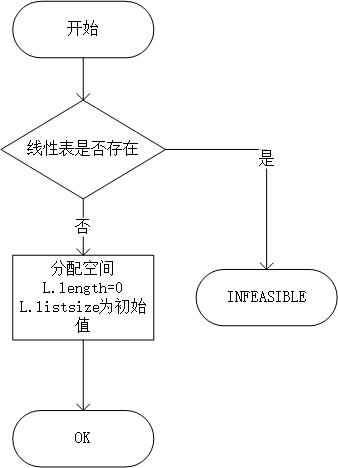
\includegraphics[scale=1]{./images/顺序表/init.jpg}
		\caption{初始化线性表流程图}
		\label{fig1-1}
	\end{center}
\end{figure}

2.销毁线性表

函数名称:DestroyList。

初始条件:线性表L已存在。

操作结果:销毁线性表L。

算法思路:若线性表存在,释放内存并将各数据设置为初值,图\ref{fig1-2}为DestroyList的流程图。
\begin{figure}[htb] % here top bottom
	\begin{center}
		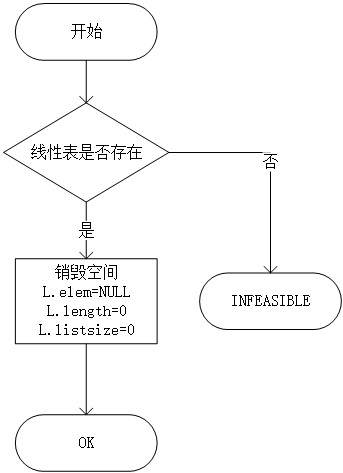
\includegraphics[scale=1]{./images/顺序表/destroy.jpg}
		\caption{初始化线性表流程图}
		\label{fig1-2}
	\end{center}
\end{figure}

\newpage

3.清空线性表

函数名称:ClearList。

初始条件:线性表L已存在。

操作结果:将L重置为空表。

算法思路:若线性表存在,则将长度设置为0即可。图\ref{fig1-3}为ClearList的流程图。
\begin{figure}[htb] % here top bottom
	\begin{center}
		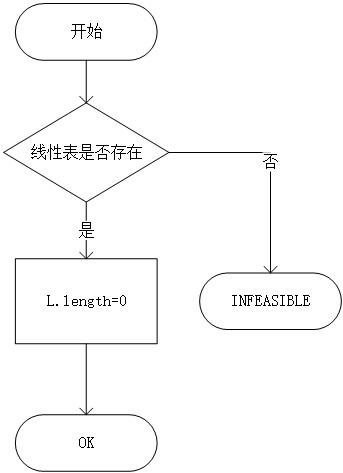
\includegraphics[scale=0.9]{./images/顺序表/clear.jpg}
		\caption{清空线性表流程图}
		\label{fig1-3}
	\end{center}
\end{figure}

\newpage

4.判断空线性表

函数名称:ListEmpty。

初始条件:线性表L已存在。

操作结果:若L为空表则返回TRUE,否则返回FALSE。

算法思路:若线性表存在,则检验L.length是否为0即可。图\ref{fig1-4}为ListEmpty的流程图。
\begin{figure}[htb] % here top bottom
	\begin{center}
		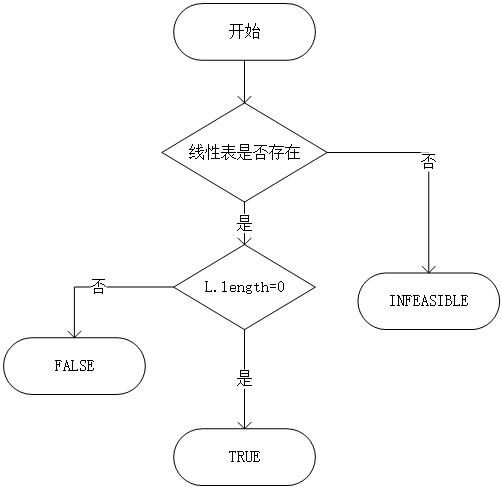
\includegraphics[scale=0.8]{./images/顺序表/empty.jpg}
		\caption{判断空线性表流程图}
		\label{fig1-4}
	\end{center}
\end{figure}

5.求线性表长

函数名称:ListLength。

初始条件:线性表L已存在。

操作结果:返回L中数据元素的个数。

算法思路:若线性表存在,直接返回表长即可。图\ref{fig1-5}是ListLength的流程图。
\begin{figure}[htb] % here top bottom
	\begin{center}
		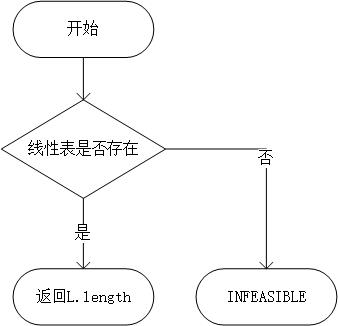
\includegraphics[scale=0.9]{./images/顺序表/length.jpg}
		\caption{求线性表长流程图}
		\label{fig1-5}
	\end{center}
\end{figure}

6.获得线性表元素

函数名称:GetElem。

初始条件:线性表L已存在。

操作结果:用e返回L中第i个数据元素的值。

算法思路:若线性表存在,返回L.elem[i-1]即可。图\ref{fig1-6}是获得线性表元素的流程图。
\begin{figure}[htb] % here top bottom
	\begin{center}
		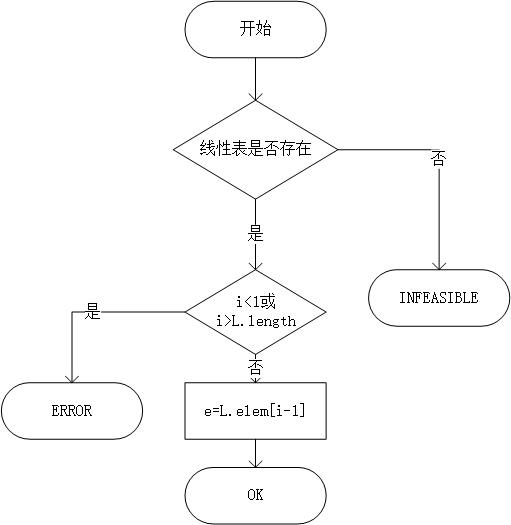
\includegraphics[scale=1]{./images/顺序表/getelem.jpg}
		\caption{获得线性表元素流程图}
		\label{fig1-6}
	\end{center}
\end{figure}

\newpage

7.查找元素

函数名称:LocateElem。

初始条件:线性表L已存在。

操作结果:返回L中第1个与e满足关系compare()关系的数据元素的位序,若这样的数据元素不存在,则返回值为0。

算法思路:若线性表存在,遍历线性表找到值为e的点,返回其下标值加一即可。图\ref{fig1-7}为查找元素的流程图。
\begin{figure}[htb] % here top bottom
	\begin{center}
		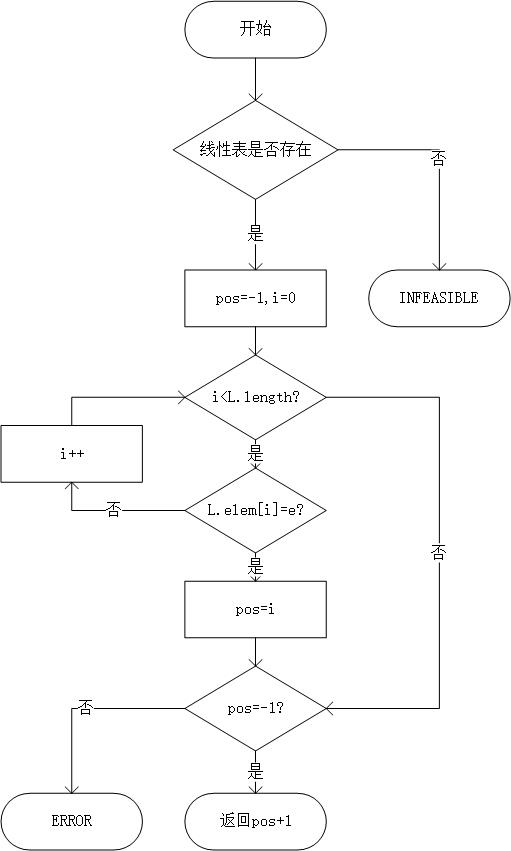
\includegraphics[scale=0.9]{./images/顺序表/locate.jpg}
		\caption{查找元素流程图}
		\label{fig1-7}
	\end{center}
\end{figure}

\newpage

8.获得前驱

函数名称:PriorElem。

初始条件:线性表L已存在。

操作结果:若e是L的数据元素,且不是第一个,则用pre返回它的前驱,否则操作失败,pre无定义。

算法思路:若线性表存在,对其从第二个数进行遍历,把L.elem[i-1]的值赋给pre即可。图\ref{fig1-8}是获得前驱的流程图。
\begin{figure}[htb] % here top bottom
	\begin{center}
		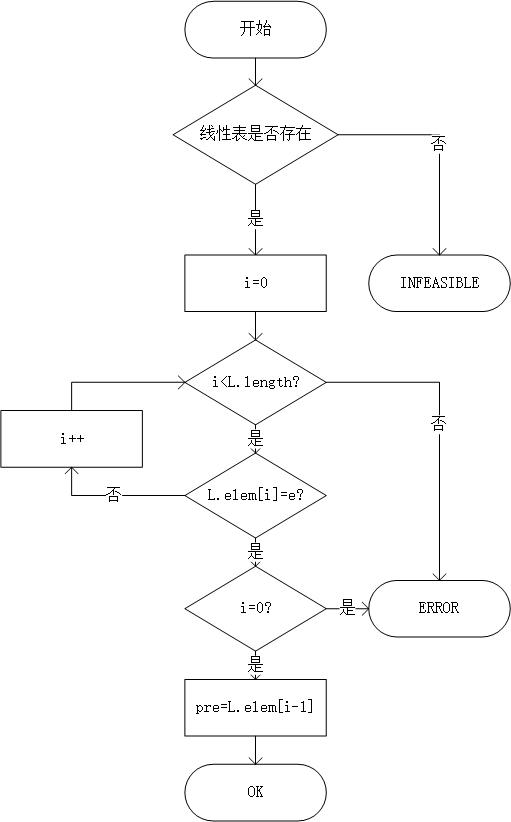
\includegraphics[scale=0.9]{./images/顺序表/prior.jpg}
		\caption{获得前驱流程图}
		\label{fig1-8}
	\end{center}
\end{figure}

\newpage


9.获得后继

函数名称:NextElem。

初始条件:线性表L已存在。

操作结果:若e是L的数据元素,且不是最后一个,则用next返回它的后继,否则操作失败,next无定义。

算法思路:若线性表存在,对其进行遍历直至倒数第二个数,把L.elem[i+1]的值赋给next即可。图\ref{fig1-9}是获得后继的流程图。
\begin{figure}[htb] % here top bottom
	\begin{center}
		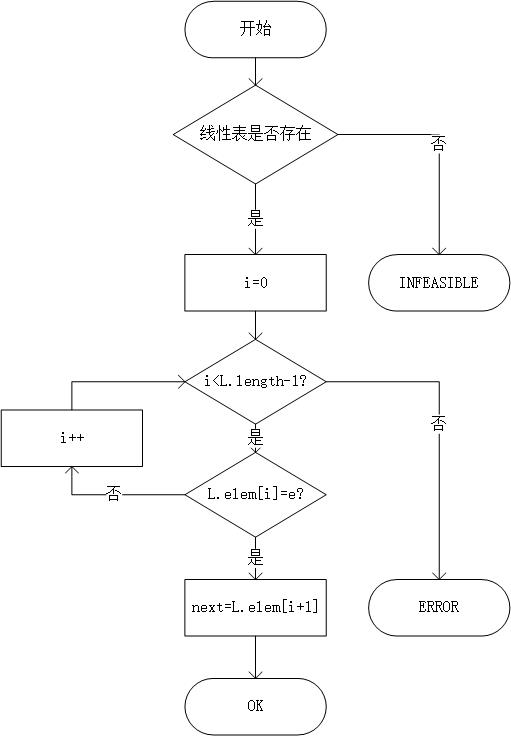
\includegraphics[scale=0.9]{./images/顺序表/next.jpg}
		\caption{获得后继流程图}
		\label{fig1-9}
	\end{center}
\end{figure}

\newpage

10.插入元素

函数名称:ListInsert。

初始条件:线性表L已存在。

操作结果:在L的第i个位置之前插入新的数据元素e。

算法思路:若线性表存在且下标合法,那么线性表第i个位置后的元素向后移一位,在第i个位置插入该数即可。图\ref{fig1-10}是插入元素的流程图。
\begin{figure}[htb] % here top bottom
	\begin{center}
		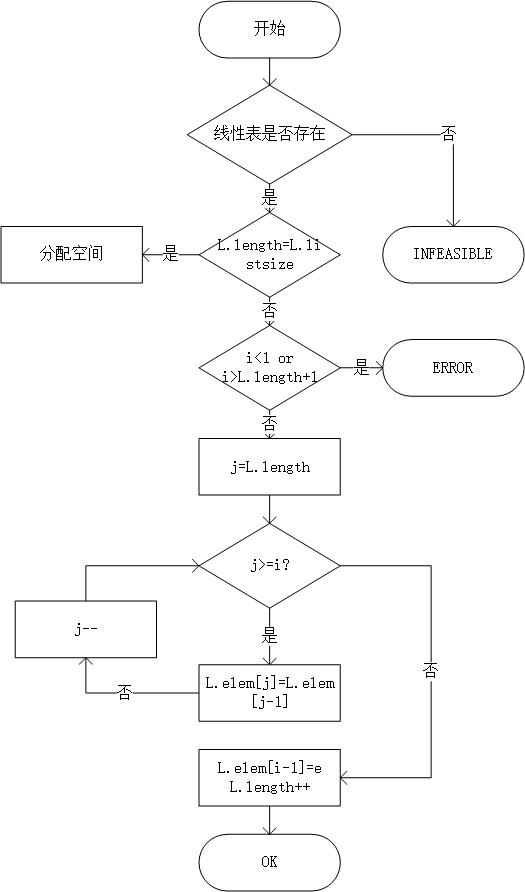
\includegraphics[scale=0.9]{./images/顺序表/insert.jpg}
		\caption{插入元素流程图}
		\label{fig1-10}
	\end{center}
\end{figure}

\newpage

11.删除元素

函数名称:ListDelete。

初始条件:线性表L已存在。

操作结果:删除L的第i个数据元素,用e返回删除的值。

算法思路:若线性表存在,则将第i个位置之后的元素向前移一位即可。图\ref{fig1-11}是删除元素的流程图。
\begin{figure}[htb] % here top bottom
	\begin{center}
		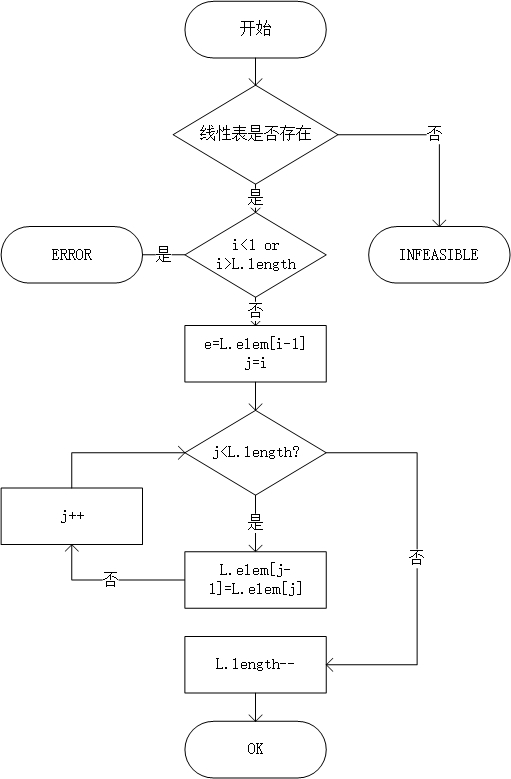
\includegraphics[scale=0.9]{./images/顺序表/delete.jpg}
		\caption{删除元素流程图}
		\label{fig1-11}
	\end{center}
\end{figure}

\newpage

12.遍历线性表

函数名称:ListTraverse。

初始条件:线性表L已存在。

操作结果:依次访问L的每个数据元素。

算法思路:若线性表存在,从第一个位置遍历到最后一个位置即可。图\ref{fig1-12}是遍历线性表的流程图。
\begin{figure}[htb] % here top bottom
	\begin{center}
		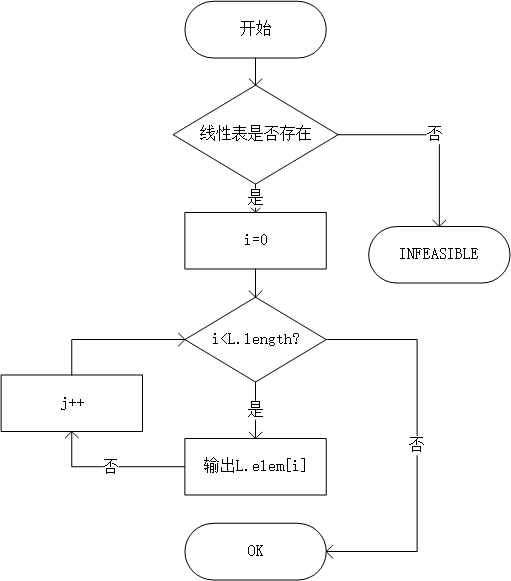
\includegraphics[scale=0.9]{./images/顺序表/traverse.jpg}
		\caption{遍历线性表流程图}
		\label{fig1-12}
	\end{center}
\end{figure}

13.最大连续子数组和

函数名称:MaxSubArray。

初始条件:线性表L已存在。

操作结果:找出一个具有最大和的连续子数组(子数组最少包含一个元素),操作结果是其最大和。

\begin{shaded*}\begin{alg}{求最大连续子数组和}
	\label{alg:1}
	\begin{algorithmic}
		\Input List $L$
		\Output the sum of max subarray
		\Procedure{MaxSubArray}{$L$}
		\For{$i=0 \rightarrow L.length$}
		\State sum += L.elem[i]
		\State ans=max(sum,ans)
		\If{$sum < 0$}
		\State $sum = 0$
		\EndIf
		\EndFor
		\State \Return $ans$
		\EndProcedure
	\end{algorithmic}
\end{alg}\end{shaded*}

14.和为K的子数组

函数名称:SubArrayNum

初始条件:线性表L已存在。

操作结果:返回该数组中和为k的连续子数组的个数。

\begin{shaded*}\begin{alg}{和为K的子数组}
	\label{alg:2}
	\begin{algorithmic}
		\Input {List $L$, int $k$}
		\Output the num of array with sum of k
		\Procedure{SubArrayNum}{$L$,$k$}
		\For{$start=0 \rightarrow L.length$}
		\State sum = 0
		\For{$end=start \rightarrow 0$}
		\State sum+=L.elem[end]
		\If{sum=k}
		\State cnt++
		\EndIf
		\EndFor
		\EndFor
		\State \Return $cnt$
		\EndProcedure
	\end{algorithmic}
\end{alg}\end{shaded*}

15.顺序表排序

函数名称:SortList

初始条件:线性表L已存在。

操作结果:将L由小到大排序。

\begin{shaded*}\begin{alg}{顺序表排序}
	\label{alg:3}
	\begin{algorithmic}
		\Input {List $L$}
		\Output L from small to large
		\Procedure{SortList}{$L$}
		\For{$i=0 \rightarrow L.length$}
		\For{$j=1 \rightarrow L.length-i$}
		\If{L.elem[j]<L.elem[j-1]}
		\State swap(L.elem[j],L.elem[j-1])
		\EndIf
		\EndFor
		\EndFor
		\State \Return $OK$
		\EndProcedure
	\end{algorithmic}
\end{alg}\end{shaded*}

16.顺序表的文件形式储存

本功能主要包括两个函数SaveList和LoadList,分别用于储存线性表到文件和读取文件中的线性表。

对于SaveList函数,若线性表存在,则先将当前线性表的元素个数和元素空间大小输入到文件中,然后将线性表中的元素按物理顺序输入即可。

对于LoadList函数,若当前线性表不存在,则可进行读取操作,先读入文件中保存的顺序表的空间大小和元素个数,分配相同的空间后,依次读入文件中顺序表的元素即可。

17.实现多个线性表管理

本功能主要包括三个函数AddList、RemoveList和LocateList,分别用于添加线性表、移除线性表和定位线性表。

对于AddList函数,若输入的名称不重复,则新建一个顺序表,长度加一,长度和空间赋值为0。

对于RemoveList函数,若存在线性表的名称与用户输入的名称相同,则将其从多表系统中移除,将序号大于该表的线性表前移一位,长度减一即可。

对于LocateList函数,若存在线性表的名称与用户输入的名称相同,则将该表的序号赋给用户操作的线性表的指针。

\subsubsection{程序源代码}
见《附录A 基于顺序存储结构线性表实现的源程序》

\newpage

\subsection{系统测试}

%主要说明针对各个函数正常和异常的测试用例及测试结果画图说明网页的整体框架,进行简要的文字描述等。画图说明网页的整体框架,进行简要的文字描述等。画图说明网页的整体框架,进行简要的文字描述等。画图说明网页的整体框架,进行简要的文字描述等。画图说明网页的整体框架,进行简要的文字描述等。画图说明网页的整体框架,进行简要的文字描述等。画图说明网页的整体框架,进行简要的文字描述等。
% \begin{figure}[htb] % here top bottom
% 	\begin{center}
% 		\includegraphics[scale=0.80]{images/1-1.pdf}
% 		\caption{网页整体框架举例}
% 		\label{fig1-1}
% 	\end{center}
% \end{figure}

% 打开EXE可执行文件,首先可以看到上方的菜单和下方空白的操作面板。上方菜单被分为两部分,上半部分为基础功能,下半部分为进阶功能。

% 打开EXE文件如图\ref{fig1-10},没有错位等现象发生,表示UI界面设计无误。
% \begin{figure}[htb] % here top bottom
% 	\begin{center}
% 		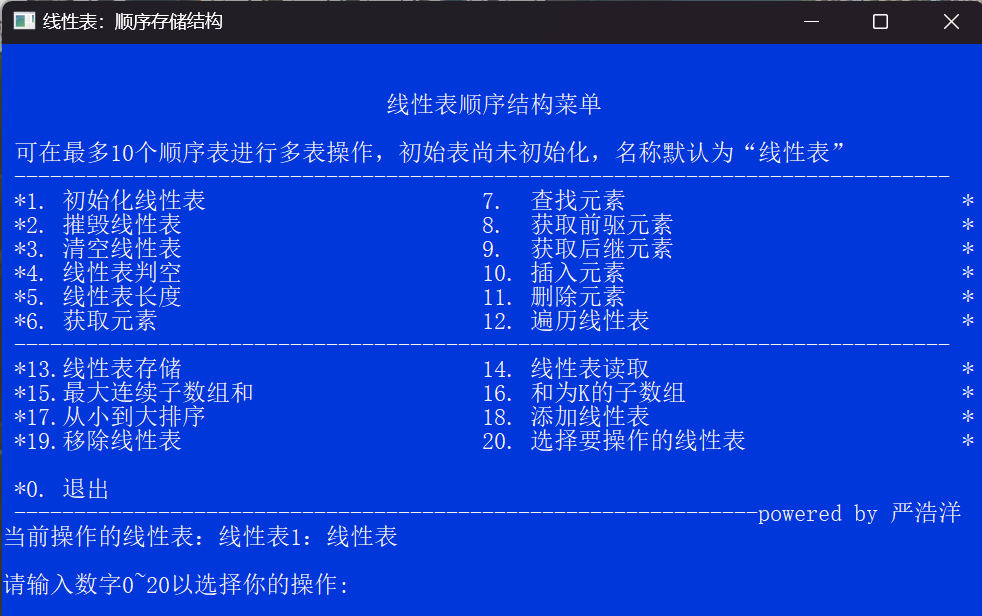
\includegraphics[scale=0.80]{./images/顺序表/0initpage.png}
% 		\caption{程序界面截图}
% 		\label{fig1-10}
% 	\end{center}
% \end{figure}

下面依次对重要功能进行测试,测试样例包括
\begin{enumerate}
	\item list1\{1,2,-4,4,5,-5,-3,-4\}
	\item null(空表)
	\item 线性表不存在
\end{enumerate}

\newpage

\begin{enumerate}
	\item 清空线性表与线性表判空的测试

	对list1进行判空操作,然后清空list1,再进行一次判空,最后销毁list1,此时线性表不存在,再进行一次判空。测试数据如表\ref{table1}所示。
	\begin{table}
		\begin{center}
		\setlength{\tabcolsep}{1.8mm}
		\caption{线性表清空与线性表判空测试表}
		\label{table1}
			\begin{tabular}{c|c|c|c}
			\hline
			测试用例    			     & 输入               & 理论结果         & 测试结果\\
			\hline
			\hline			
			\multirow{5}{*}{list1}   	& 4              	 & 线性表不为空!   & 线性表不为空!\\
										& 3              	 & 已清空线性表!   & 已清空线性表!\\
										& 4			         & 线性表为空!   	& 线性表为空!\\
										& 2				     & 已销毁线性表!   & 已销毁线性表!\\
										& 4				     & 判断失败!线性表不存在!   & 判断失败!线性表不存在!\\
			\hline
			\end{tabular}
		\end{center}
	\end{table}

	测试结果如下图\ref{fig1-13}所示。
	\begin{figure}[htb] % here top bottom
		\begin{center}
			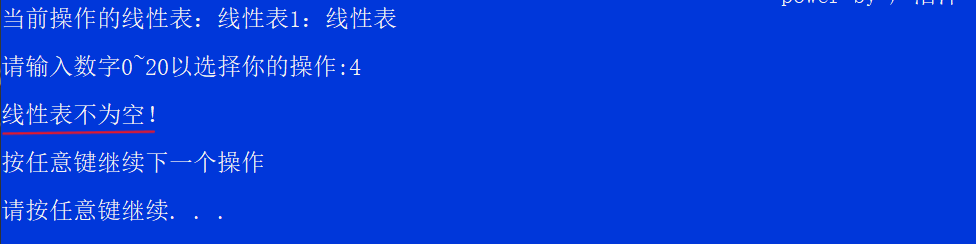
\includegraphics[scale=0.6]{./images/顺序表/4ori.png}
			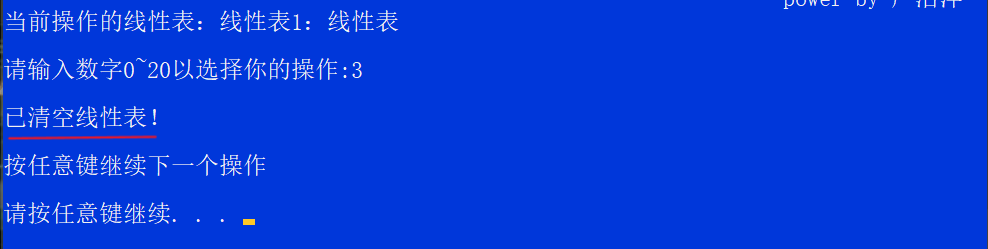
\includegraphics[scale=0.6]{./images/顺序表/3list1.png}
			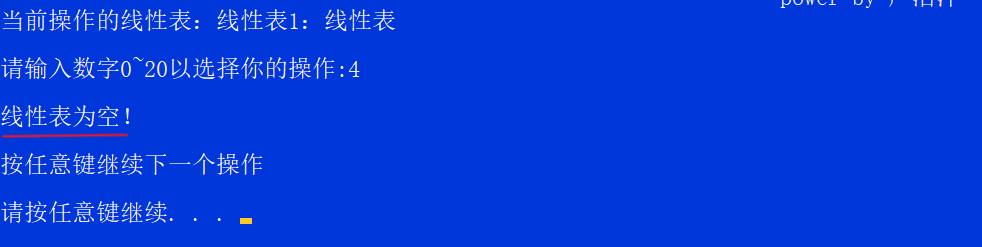
\includegraphics[scale=0.6]{./images/顺序表/43.png}
			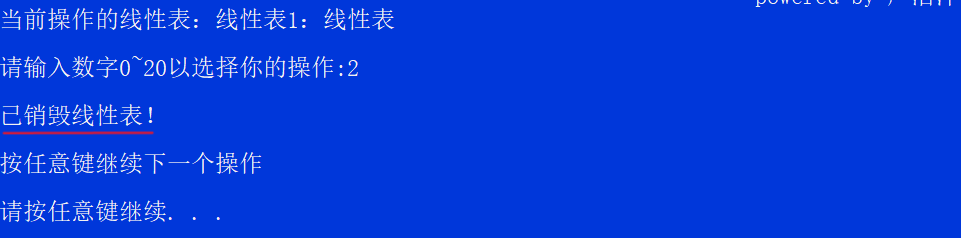
\includegraphics[scale=0.6]{./images/顺序表/2.png}
			\caption{清空线性表与线性表判空测试组的截图}
			\label{fig1-13}
		\end{center}
	\end{figure}

	\newpage

	\item 获得、查找元素及其前驱后继的测试
	
	对list1进行获得第三个元素的操作,然后对其进行查找并获取其前驱后继。测试数据如表\ref{table2}所示。
	\begin{table}
		\begin{center}
		\setlength{\tabcolsep}{2.0mm}
		\caption{获得、查找元素及其前驱后继测试表}
		\label{table2}
			\begin{tabular}{c|c|c|c}
			\hline
			测试用例    			     & 输入               & 理论结果         & 测试结果\\
			\hline
			\hline			
			\multirow{4}{*}{list1}   	& 6 3              	 & 获取元素值为-4   & 获取元素值为-4\\
										& 7 -4             	 & 查找元素在第3个  & 查找元素在第3个\\
										& 8	-4		         & 查询元素前驱为2  & 查询元素前驱为2\\
										& 9	-4			     & 查询元素后继为4  & 查询元素后继为4\\
			\hline
			\end{tabular}
		\end{center}
	\end{table}

	测试结果如下图\ref{fig1-14}所示。
	\begin{figure}[htb] % here top bottom
		\begin{center}
			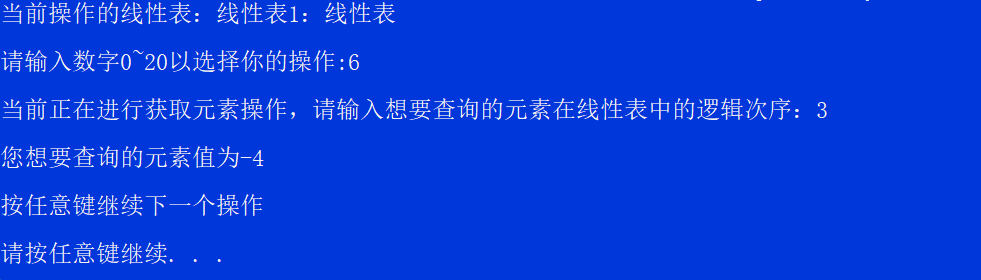
\includegraphics[scale=0.6]{./images/顺序表/6.png}
			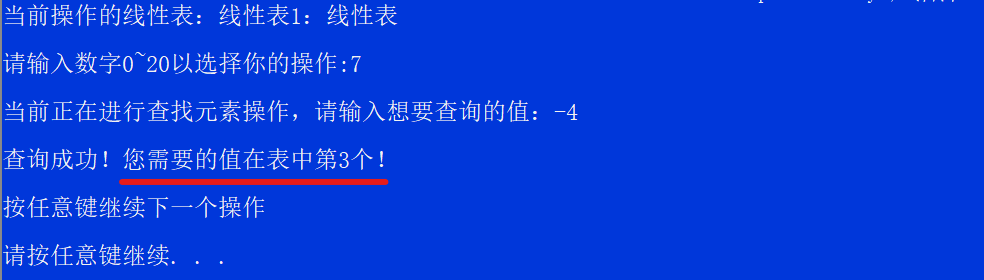
\includegraphics[scale=0.6]{./images/顺序表/7.png}
			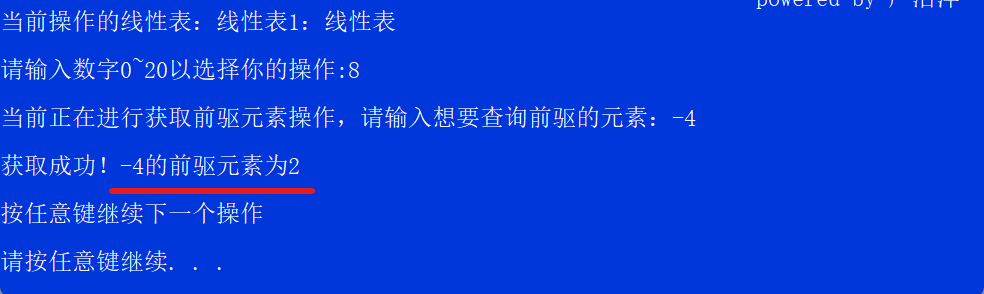
\includegraphics[scale=0.6]{./images/顺序表/8.png}
			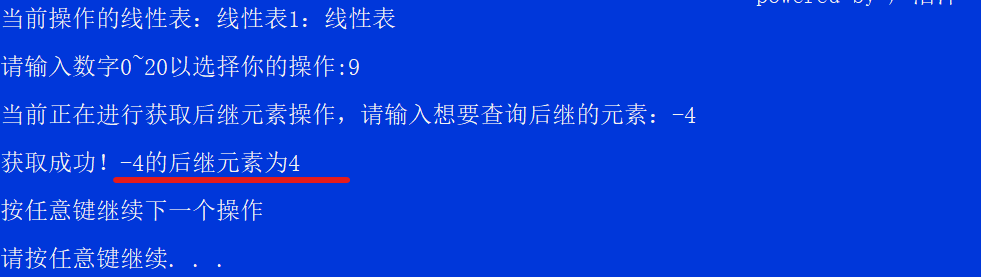
\includegraphics[scale=0.6]{./images/顺序表/9.png}
			\caption{获得、查找元素及其前驱后继测试组的截图}
			\label{fig1-14}
		\end{center}
	\end{figure}

	除标准数据外,下面测试了一些不合法数据、临界数据,依次为输入下标不合法、获取元素不在线性表中、获取前驱的元素为表头、获取后继的元素不在线性表中的情况。测试结果如下图\ref{fig1-15}所示。
	\begin{figure}[htb] % here top bottom
		\begin{center}
			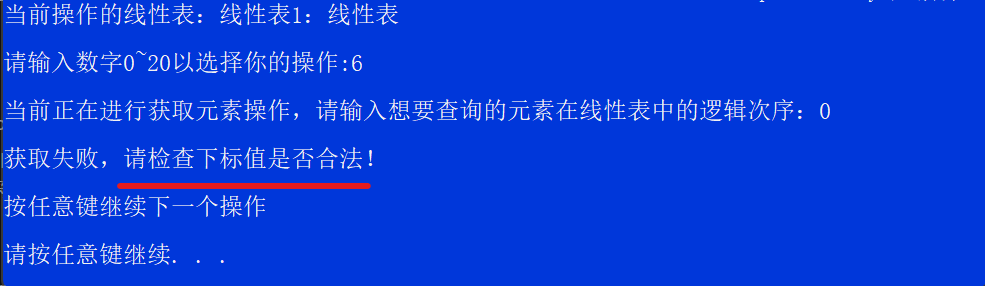
\includegraphics[scale=0.6]{./images/顺序表/2_1.png}
			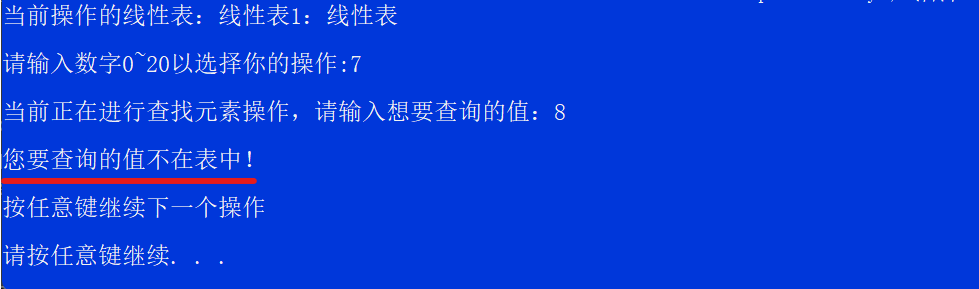
\includegraphics[scale=0.6]{./images/顺序表/2_2.png}
			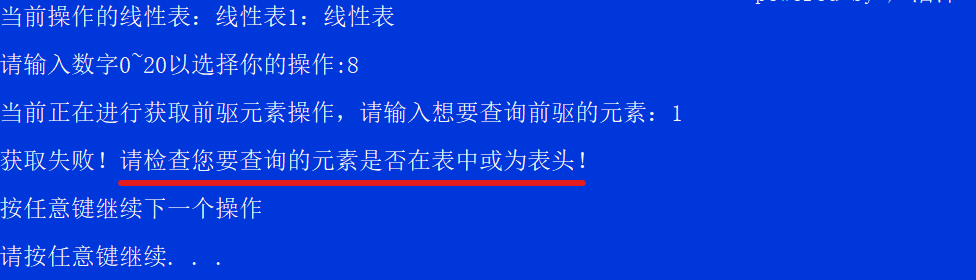
\includegraphics[scale=0.6]{./images/顺序表/2_3.png}
			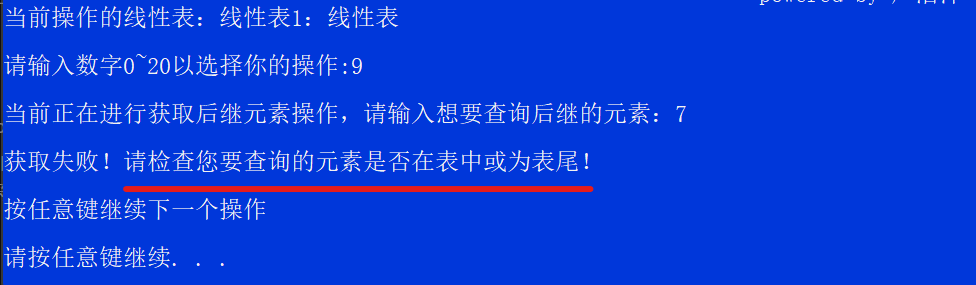
\includegraphics[scale=0.6]{./images/顺序表/2_4.png}
			\caption{不合法数据、临界数据的测试}
			\label{fig1-15}
		\end{center}
	\end{figure}

	以上结果均符合预期。

	\newpage

	\item 插入、删除、遍历元素的测试
	对list1依次进行插入、删除和遍历操作,测试数据如表\ref{table3}所示。
	\begin{table}
		\begin{center}
		\setlength{\tabcolsep}{2.0mm}
		\caption{插入、删除、遍历元素测试表}
		\label{table3}
			\begin{tabular}{c|c|c|c}
			\hline
			测试用例    			     & 输入               & 理论结果         & 测试结果\\
			\hline
			\hline			
			\multirow{4}{*}{list1}   	& 10 3 2           	 & 插入成功!       & 插入成功!\\
										& 12		         & 1 2 2 -4 4 5 -5 -3 -4  & 1 2 2 -4 4 5 -5 -3 -4\\
										& 11 3             	 & 删除的元素为2    & 删除的元素为2\\
										& 12			     & 1 2 -4 4 5 -5 -3 -4   & 1 2 -4 4 5 -5 -3 -4\\
			\hline
			\end{tabular}
		\end{center}
	\end{table}

	测试结果如下图\ref{fig1-16}、图\ref{fig1-17}所示。
	\begin{figure}[htb] % here top bottom
		\begin{center}
			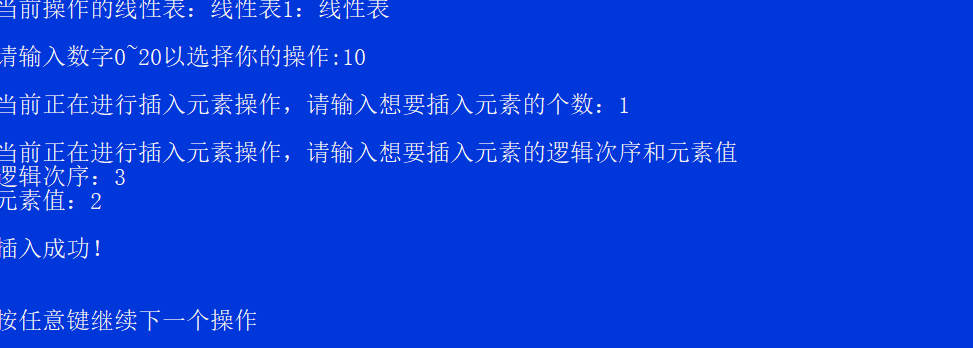
\includegraphics[scale=0.6]{./images/顺序表/10.png}
			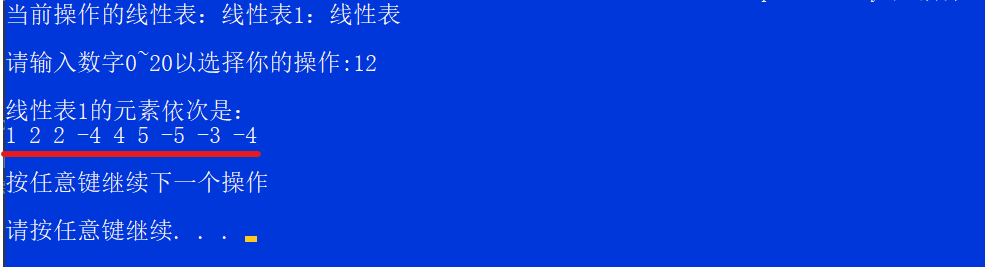
\includegraphics[scale=0.6]{./images/顺序表/12_1.png}
			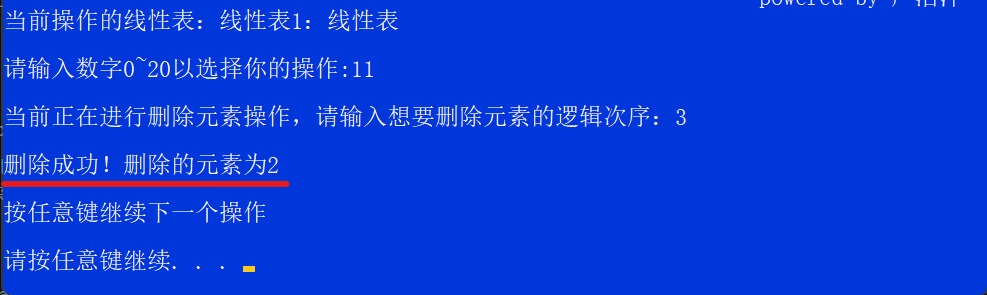
\includegraphics[scale=0.6]{./images/顺序表/11.png}
			\caption{插入、删除、遍历元素测试组的截图(1)}
			\label{fig1-16}
		\end{center}
	\end{figure}
	\begin{figure}[htb] % here top bottom
		\begin{center}
			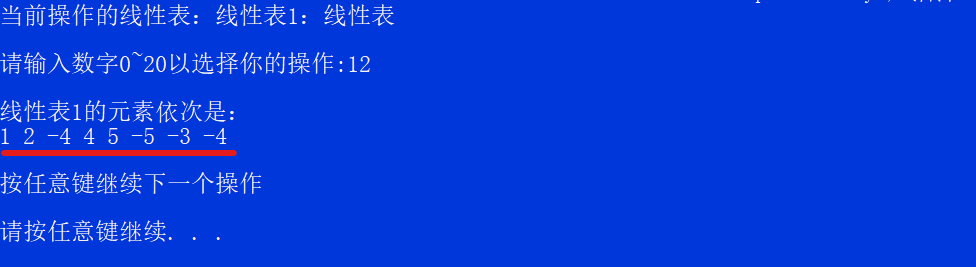
\includegraphics[scale=0.6]{./images/顺序表/12_2.png}
			\caption{插入、删除、遍历元素测试组的截图(2)}
			\label{fig1-17}
		\end{center}
	\end{figure}

	\newpage

	除标准数据外,下面测试了一些不合法数据、临界数据,依次为插入、删除下标不合法,线性表不存在的情况。测试结果下图\ref{fig1-18}所示。
	\begin{figure}[htb] % here top bottom
		\begin{center}
			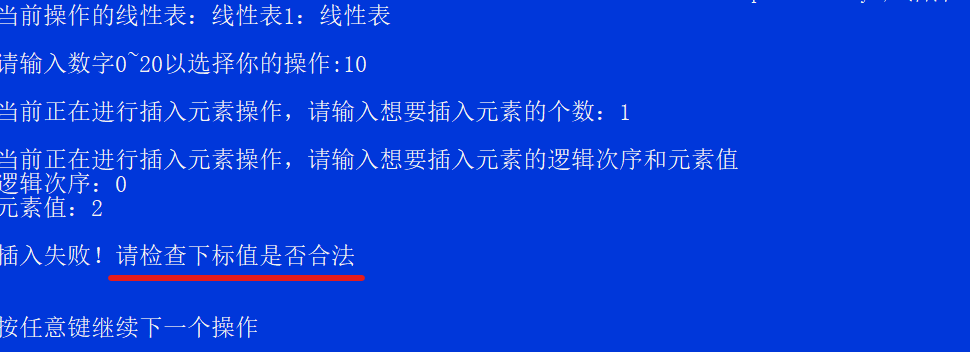
\includegraphics[scale=0.6]{./images/顺序表/3_1.png}
			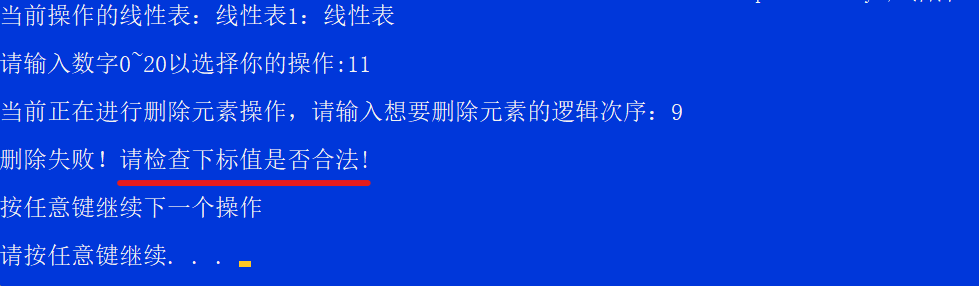
\includegraphics[scale=0.6]{./images/顺序表/3_2.png}
			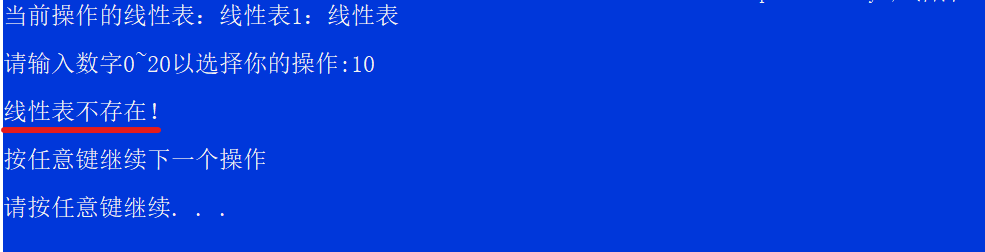
\includegraphics[scale=0.6]{./images/顺序表/3_3.png}
			\caption{不合法数据、临界数据的测试}
			\label{fig1-18}
		\end{center}
	\end{figure}

	以上结果均符合预期。
\end{enumerate}
\newpage
% 下面是将五次实验截图的组图\ref{fig1-11}。
% \begin{figure}[htb] % here top bottom
% 	\begin{center}
% 		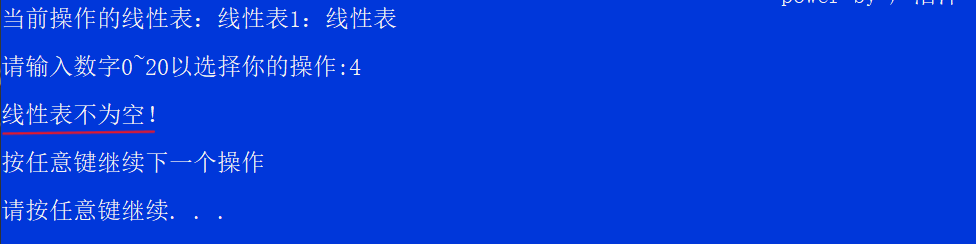
\includegraphics[scale=0.80]{./images/顺序表/4ori.png}
% 		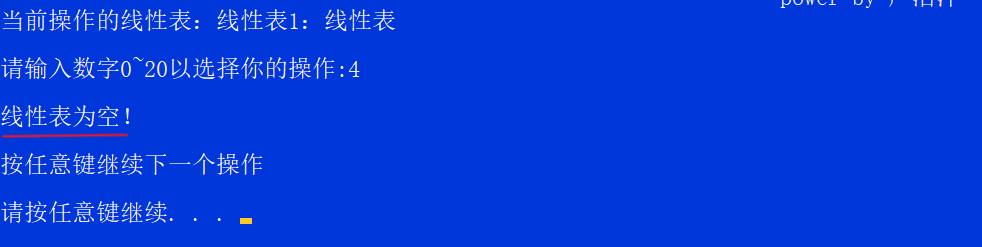
\includegraphics[scale=0.80]{./images/顺序表/43.png}
% 		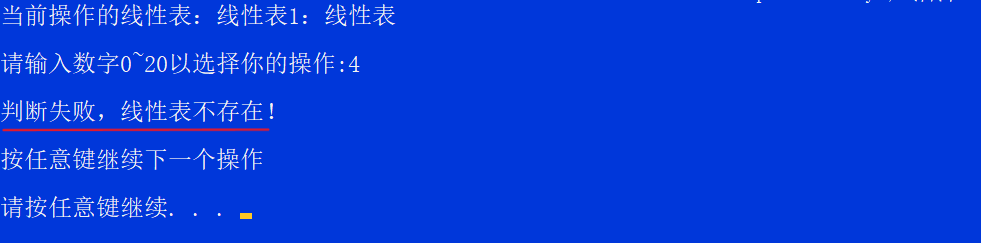
\includegraphics[scale=0.80]{./images/顺序表/24.png}
% 		\caption{清空线性表与线性表判空测试组的截图}
% 		\label{fig1-11}
% 	\end{center}
% \end{figure}

\subsection{实验小结}

本次实验以实现顺序表的逻辑结构及其功能为主要目的。基础功能整体难度不大,附加功能中,多线性表管理较为复杂,最大连续子数组和、和为K的子数组等功能在基础算法方面也有一定的要求。

这次实验中我学习并练习了许多东西。最大连续子数组和题目中,我首先使用动态规划进行实现,后来我学习并使用了在线处理这一算法,有效降低了算法的空间复杂度。顺序表排序中,我也练习了《数据结构》课程第十章中的多种排序方法。文件存取和多线性表管理的功能也让我复习了上学期《C语言程序设计》课程中学到的结构与文件的知识。为美化程序界面,我学习了一些关于system函数的知识,改变了程序框的大小和颜色。

本次实验中我也有一些常见的错误。在进行多线性表管理时,常常会错误地判断线性表个数,这是由于在相关功能上不能正确地增减线性表个数,如“初始化线性表”、“销毁线性表”、“读取线性表”、“添加/移除线性表”等等。最终建立了正确合理的增减线性表数目的规则。在设计系统主体时,我没有首先考虑后期多线性表管理的实现,后期再进行删改,耗费了一些时间。

编写实验报告时,我复习了visio画流程图的方法,学习了使用伪代码描述算法的格式,锻炼了综合能力,为将来的科研奠定了基础。

\newpage

% 重点说明在实验中取得的实际经验,例如调试中碰到的典型错误等,不要写套话。画图说明网页的整体框架,进行简要的文字描述等。画图说明网页的整体框架,进行简要的文字描述等。画图说明网页的整体框架,进行简要的文字描述等。画图说明网页的整体框架,进行简要的文字描述等。画图说明网页的整体框架,进行简要的文字描述等。画图说明网页的整体框架,进行简要的文字描述等。画图说明网页的整体框架,进行简要的文字描述等。

% \begin{figure}[htb]
% 	\begin{center}
% 		\includegraphics[scale=0.60]{images/1-2.png}
% 		\caption{在visio里通过文件-打印,把visio图打印成pdf文件}
% 		\label{fig1-2}
% 	\end{center}
% \end{figure}

% 画图说明网页的整体框架,进行简要的文字描述等。画图说明网页的整体框架,进行简要的文字描述等。画图说明网页的整体框架,进行简要的文字描述等。画图说明网页的整体框架,进行简要的文字描述等。画图说明网页的整体框架,进行简要的文字描述等。画图说明网页的整体框架,进行简要的文字描述等。画图说明网页的整体框架,进行简要的文字描述等。

% \begin{figure}[htb]
% 	\begin{center}
% 		\includegraphics[scale=0.50]{images/1-3.png}
% 		\caption{用pdf阅览器的工具,对打印得到pdf图做适当的裁剪}
% 		%\label{fig1-3}
% 	\end{center}
% \end{figure}

% 其实吧,用Latex写公式也不是很难,请参照公式\ref{equ_loss}。画表格就更简单了,请看表\ref{table2}。

% \begin{eqnarray}\label{equ_loss}
% 	\mathcal{L}_{id}=\sum_{j=1}^{c}1\{l_k=j\}\log\frac{\exp(f_j(\textbf{W},x_k))}{\sum\nolimits_{l=1}^{c}\exp(f_l(\textbf{W},x_k))}
% \end{eqnarray}

% 画图说明网页的整体框架,进行简要的文字描述等。画图说明网页的整体框架,进行简要的文字描述等。画图说明网页的整体框架,进行简要的文字描述等。画图说明网页的整体框架,进行简要的文字描述等。画图说明网页的整体框架,进行简要的文字描述等。画图说明网页的整体框架,进行简要的文字描述等。画图说明网页的整体框架,进行简要的文字描述等。

% \begin{table}
% 	\begin{center}
% 		\setlength{\tabcolsep}{2.0mm}
% 		\caption{Mean and standard deviation of estimation error (Euler angles) on Pandora. The best performance is in \textbf{bold}.}
% 		\label{table2}
% 		\begin{tabular}{c|ccccc}
% 			\hline
% 			Method    			        & Data               & Pitch         & Roll           & Yaw              & Accuracy\\
% 			\hline
% 			\hline			
% 			\multirow{5}{*}{POSEidon}   & Depth              & 6.5 $\pm$ 6.6  & 5.4 $\pm$ 5.1  & 10.4 $\pm$ 11.8  & 0.646\\
% 			& FfD              	 & 6.8 $\pm$ 7.0  & 5.7 $\pm$ 5.7  & 10.5 $\pm$ 14.6  & 0.647\\
% 			& Gray-level         & 7.1 $\pm$ 6.6  & 5.6 $\pm$ 5.8  & 9.0  $\pm$ 10.9  & 0.639\\
% 			& Depth + FfD	     & 5.6 $\pm$ 5.0  & 4.9 $\pm$ 5.0  & 9.8  $\pm$ 13.4  & 0.698\\
% 			& Depth + FfD + MI   & 5.7 $\pm$ 5.6  & 4.9 $\pm$ 5.1  & 9.0  $\pm$ 11.9  & 0.715\\
% 			\hline
% 			DRF                         & Depth              & 6.2 $\pm$ 9.5  & 4.6 $\pm$ 6.7  & 9.3  $\pm$ 14.6  & --\\
% 			\hline
% 			\multirow{3}{*}{Ours}   	& Depth              & 5.9 $\pm$ 6.2  & 4.5 $\pm$ 4.9  & 8.8  $\pm$ 10.9  & 0.666\\
% 			& RGB                & 5.5 $\pm$ 5.3  & 4.4 $\pm$ 5.5  & 8.6  $\pm$ 9.3   & 0.698\\
% 			& RGB + Depth        & 5.0 $\pm$ 4.8  & 4.3 $\pm$ 4.9  & 8.1  $\pm$ 8.3   & \textbf{0.737}\\
% 			\hline
% 		\end{tabular}
% 	\end{center}
% \end{table}

\section{基于邻接表的图实现}

% 描述主页的结构,给出主页截图,描述主要设计思路等,请见图\ref{fig2-1}。描述主页的结构,给出主页截图,描述主要设计思路等。描述主页的结构,给出主页截图,描述主要设计思路等。描述主页的结构,给出主页截图,描述主要设计思路等。描述主页的结构,给出主页截图,描述主要设计思路等。描述主页的结构,给出主页截图,描述主要设计思路等。描述主页的结构,给出主页截图,描述主要设计思路等。

% \begin{figure}[htb]
% 	\begin{center}
% 		\includegraphics[scale=0.40]{images/2-1.jpg}
% 		\caption{主页举例}
% 		\label{fig2-1}
% 	\end{center}
% \end{figure}

\subsection{问题描述}

实验要求以邻接表的形式实现图这一数据结构,并创建一个菜单来实现功能的演示。功能包括\textbf{基础的}创建、销毁与增删改查等操作,其中增删包括结点与弧的增删,搜索包括常见的深度优先搜索(DFS)与广度优先搜索(BFS),以及进阶的文件存取、多图管理与距离小于k的顶点集合、最短路径等使用功能。

\subsubsection{功能实现}

具体实现的功能如下:

\begin{enumerate}
	\item 基础功能
		\begin{enumerate}
			\item 创建图
			\item 销毁图
			\item 查找顶点
			\item 顶点赋值
			\item 获得第一邻接点
			\item 获得下一邻接点
			\item 插入顶点
			\item 删除顶点
			\item 插入弧
			\item 删除弧
			\item 深度优先搜索遍历
			\item 广度优先搜索遍历
		\end{enumerate}
	\item 进阶功能
		\begin{enumerate}
			\item 距离小于k的顶点集合
			\item 顶点间最短路径和长度
			\item 图的连通分量
			\item 实现图的文件形式保存
			\item 实现多个图管理
		\end{enumerate}
\end{enumerate}

\subsubsection{实验目的}
\begin{enumerate}
	\item 加深对图的概念、基本运算的理解
	\item 熟练掌握图的逻辑结构与物理结构的关系
	\item 以邻接表作为物理结构,熟练掌握图基本运算的实现
\end{enumerate}

% 说明此实验要解决的基本问题。大力出奇迹!!!参考文献无法显示怎么办?陈老师正在想办法解决\cite{STR2021Neurocom, AVS2021Neurocom}!我是参考文献。我是第二小节\cite{Mehrabian1974An}。我是第二小节\cite{Rezaei2014CVPR}。我是第二小节\cite{Ramnath2008IJCV}。

\subsection{系统设计}

\subsubsection{系统总体设计}

本系统再初始条件下提供一个以邻接表形式存储的图,用户可自行添加新的图或移除原有的图,图的个数不超过十个。每个图之间\textbf{相互独立},均可独立实现所有的功能,也可通过“选择图”功能切换要操作的图。系统所实现的功能包括基础功能和进阶功能两部分,已在上一节列出。

系统利用一个简易菜单以供用户选择需要的功能。通过\textbf{清屏函数}等操作,并用\textbf{system}相关函数调整窗口大小,可以使菜单选项始终位于界面上方,方便用户选择。

主函数中主要包括相关变量的定义以及菜单的实现,利用\textbf{switch分支结构}以实现功能的选择,并将特定的功能分别封装于不同的函数中。在主函数中只需调用相应函数即可。

\subsubsection{数据结构设计}

本实验使用了多个结构体以定义图的各个部分,包括:
\begin{enumerate}
	\item VertexType:表示图的结点
	\item ArcNode:表示邻接表结点,即表示弧
	\item VNode:表示头节点
	\item ALGraph:表示图
\end{enumerate}

除以上图的相关定义外,本实验沿用顺序表的结构:Lists,以实现多图管理。

% 包括整体系统结构设计和数据结构设计等。先在文件夹里的bib文件里添加新的参考文献,给每篇参考文献取一个索引的名字,然后再引用比如\cite{STR2021Neurocom}\cite{AVS2021Neurocom, Rezaei2014CVPR}。请注意书籍、期刊论文、专利等bib条目的格式是不一样的。画图说明网页的整体框架,进行简要的文字描述等。画图说明网页的整体框架,进行简要的文字描述等。画图说明网页的整体框架,进行简要的文字描述等。画图说明网页的整体框架,进行简要的文字描述等。画图说明网页的整体框架,进行简要的文字描述等。画图说明网页的整体框架,进行简要的文字描述等。画图说明网页的整体框架,进行简要的文字描述等。

\newpage

\subsection{系统实现}

\subsubsection{算法设计}

1.创建图

函数名称:CreateGraph

初始条件:无向图G不存在,给定结点与邻接数组,结点不超过二十个。

操作结果:构造一个无向图G,要求满足各顶点关键字的唯一性。

算法思路:先计算弧与结点的个数,判断关键字是否重复、是否为空图、是否超过二十个结点,若以上情况均不存在,则对每条边使用InsertArc函数。图\ref{fig2-1}为CreateGraph的流程图。

\begin{figure}[htb] % here top bottom
	\begin{center}
		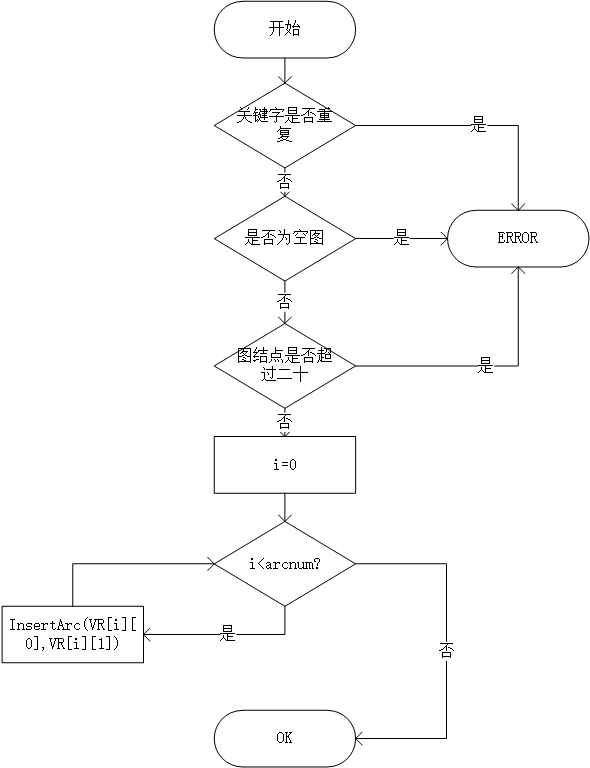
\includegraphics[scale=0.9]{./images/图/CreateGraph.jpg}
		\caption{创建图流程图}
		\label{fig2-1}
	\end{center}
\end{figure}

\newpage

2.销毁图

函数名称:DestroyGraph

初始条件:无向图G存在。

操作结果:邻接表表示的无向图销毁,并释放所有表结点的空间。

算法思路:对每一个表头结点,由firstarc开始依次释放弧结点,最后把G.vexnum、G.arcnum改为0即可。图\ref{fig2-2}为DestroyGraph的流程图。

\begin{figure}[htb] % here top bottom
	\begin{center}
		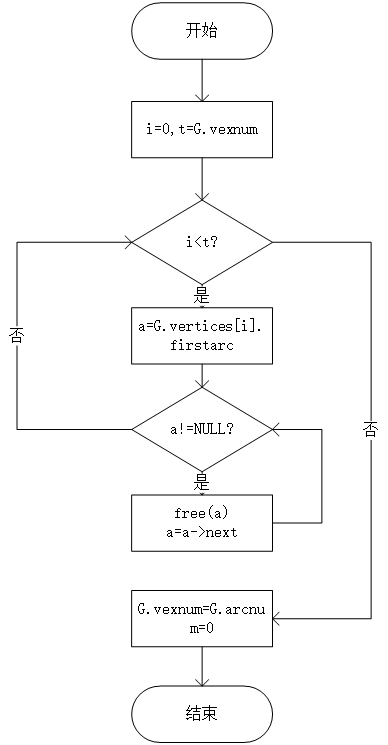
\includegraphics[scale=0.9]{./images/图/Destroy.jpg}
		\caption{销毁图流程图}
		\label{fig2-2}
	\end{center}
\end{figure}

\newpage

3.查找顶点

函数名称:LocateVex

初始条件:无向图G存在。

操作结果:成功时返回关键字为u的顶点位置序号(简称位序),否则返回-1。

算法思路:遍历每一个头节点即可,判断结点关键字是否与传入的关键字u相等,若查询成功返回当前位序,否则返回-1。图\ref{fig2-3}为LocateVex的流程图。

\begin{figure}[htb] % here top bottom
	\begin{center}
		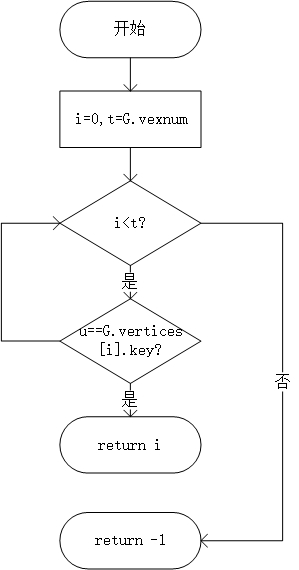
\includegraphics[scale=0.9]{./images/图/Locatevex.jpg}
		\caption{查找顶点流程图}
		\label{fig2-3}
	\end{center}
\end{figure}

\newpage

4.顶点赋值

函数名称:PutVex

初始条件:无向图G存在。

操作结果:对关键字为u的顶点赋值value(要求关键字具有唯一性)。

算法思路:先判断关键字是否重复,若不重复则遍历头结点,找到对应关键字u的点,更改关键字即可。图\ref{fig2-4}为PutVex的流程图。

\begin{figure}[htb] % here top bottom
	\begin{center}
		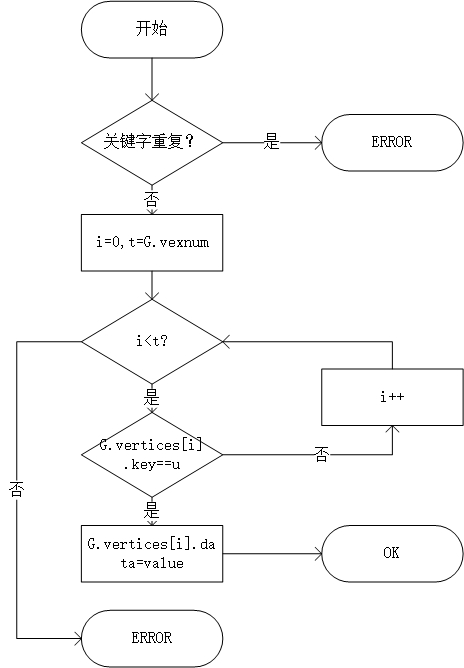
\includegraphics[scale=0.9]{./images/图/Put.jpg}
		\caption{顶点赋值流程图}
		\label{fig2-4}
	\end{center}
\end{figure}

\newpage

5.获得第一邻接点

函数名称:FirstAdjVex

初始条件:无向图G存在。

操作结果:返回关键字为u的顶点第一个邻接顶点的位序,否则返回-1。

算法思路:先判断关键字是否重复,若不重复则遍历头结点,找到对应关键字u的点,更改关键字即可。图\ref{fig2-5}为FirstAdjVex的流程图。

\begin{figure}[htb] % here top bottom
	\begin{center}
		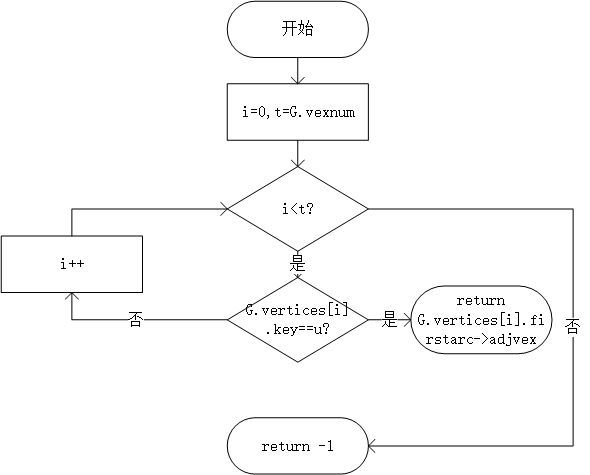
\includegraphics[scale=0.9]{./images/图/First.jpg}
		\caption{获得第一邻接点流程图}
		\label{fig2-5}
	\end{center}
\end{figure}

6.获得下一邻接点

函数名称:NextAdjVex

初始条件:无向图G存在。

操作结果:返回v相对于w的下一个邻接顶点的位序;如果w是最后一个邻接顶点,或v、w对应顶点不存在,则返回-1。

算法思路:先遍历寻找结点v,然后在v的邻接结点中寻找w。若w不是最后一个邻接结点,则返回其nextarc指向的adjvex。

7.插入顶点

函数名称:InsertVex

初始条件:无向图G存在。

操作结果:在图G中插入新顶点V,要求满足关键字唯一性。

算法思路:先判断结点数是否超出上限,关键字是否重复。然后在头节点数组末尾插入新节点,G.vexnum+1即可。图\ref{fig2-6}是InsertVex的流程图。

\begin{figure}[htb] % here top bottom
	\begin{center}
		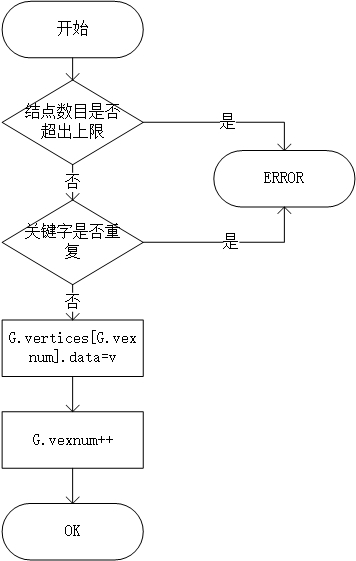
\includegraphics[scale=0.9]{./images/图/InsertVex.jpg}
		\caption{插入顶点流程图}
		\label{fig2-6}
	\end{center}
\end{figure}

8.删除顶点

函数名称:DeleteVex

初始条件:无向图G存在。

操作结果:在图G中删除关键字v对应的顶点以及相关的弧。

算法思路:先遍历头结点数组,找到关键字对应的结点,释放其所有弧结点后,将该节点后的全部结点向前移一位,G.vexnum-1。然后对每一个头结点进行遍历,遍历每个结点的所有弧结点,若找到有关联删去点的弧则释放。

9.插入弧

函数名称:InsertArc

初始条件:无向图G存在。

操作结果:在图G中增加弧<v,w>。

算法思路:先遍历头结点,找到v和w对应头结点的位序,若未找到则返回ERROR。然后新建弧结点,关联结点w,将其作为结点v的firstarc。同理可关联w到v的弧。


10.删除弧

函数名称:DeleteArc

初始条件:无向图G存在。

操作结果:在图G中删除弧<v,w>。

算法思路:先遍历头结点,找到v和w对应头结点的位序,若未找到则返回ERROR。然后遍历V的弧结点,找到关联W的弧则释放,同理释放W弧中关联V的弧结点,若未找到关联v、w的弧则返回ERROR。

11.深度优先搜索遍历

函数名称:DFSTraverse

初始条件:无向图G存在。

操作结果:对图G进行深度优先搜索遍历。

可以使用深度优先搜索(DFS)递归函数进行辅助,对每个头结点进行DFS操作,用标记数组flag记录结点是否遍历。

\begin{shaded*}\begin{alg}{深度优先搜索}
	\label{alg:4}
	\begin{algorithmic}
		\Input {ALGraph $G$,int $v$}
		\Output Elements of G in DFS sequence
		\Procedure{DFS}{$G$,$v$}
		\State arc=G.vertices[v].firstarc
		\State visit(G.vertices[v].data)
		\State flag[v]=1
		\While{arc}
			\If{!flag[arc->adjvex]}
				\State DFS(G,arc->adjvex)
			\EndIf
			\State arc=arc->nextarc
		\EndWhile
		\State \Return
		\EndProcedure
	\end{algorithmic}
\end{alg}\end{shaded*}

12.广度优先搜索遍历

函数名称:BFSTraverse

初始条件:无向图G存在。

操作结果:对图G进行广度优先搜索遍历。

可以使用队列(queue)这一数据结构进行辅助,用标记数组flag记录结点是否遍历过。

\begin{shaded*}\begin{alg}{广度优先搜索}
	\label{alg:5}
	\begin{algorithmic}
		\Input {ALGraph $G$}
		\Output Elements of G in BFS sequence
		\Procedure{DFS}{$G$}
		\For{$i=0\rightarrow G.vexnum$}
			\If{!flag[i]}
				\State visit(G.vertices[i].data)
				\State queue[tail++]=G.vertices[i].firstarc
				\While{front<tail}
					\State arc=queue[front++]
					\If{!flag[arc->adjvex]}
						\State flag[arc->adjvex]=1
						\State visit(G.vertices[arc->adjvex].data)
						\State 邻接结点全部入队
					\EndIf
				\EndWhile
			\EndIf
		\EndFor
		\State \Return
		\EndProcedure
	\end{algorithmic}
\end{alg}\end{shaded*}

13.距离小于k的顶点集合

函数名称:VerticesSetLessThanK

初始条件:无向图G存在。

操作结果:返回与顶点v距离小于k的顶点集合。

算法思路:先遍历头结点数组,找到关键字对应的结点,由于“深度”与“距离”的相似性,可以利用dfs函数递归遍历所有距离小于K的点。

14.顶点间最短路径和长度

函数名称:ShortestPathLength

初始条件:无向图G存在。

操作结果:返回顶点v与顶点w的最短路径的长度。

可以利用Floyd-Warshall算法求任意两点间最短路径,然后带入这两点的值返回即可。

\begin{shaded*}\begin{alg}{最短路径算法}
	\label{alg:6}
	\begin{algorithmic}
		\Input {ALGraph $G$,int $a$,int$b$}
		\Output the shortest length between a and b
		\Procedure{ShortestPathLength}{$G$}
		\For{$i\rightarrow G.vexnum$}
			\For{$j\rightarrow G.vexnum$}
				\For{$k\rightarrow G.vexnum$}
					\If{G[i][j]>G[i][k]+G[k][j]}
						\State G[i][j]>G[i][k]+G[k][j]
					\EndIf
				\EndFor
			\EndFor
		\EndFor
		\State \Return G[a][b]
		\EndProcedure
	\end{algorithmic}
\end{alg}\end{shaded*}

15.图的连通分量

函数名称:ConnectedComponentsNums

初始条件:无向图G存在。

操作结果:返回图G的所有连通分量的个数。

算法思路:同样利用深度优先搜素算法,从一个头结点开始遍历,遇到未遍历的头结点,则连通分量加一。

16.图的文件形式储存

本功能主要包括两个函数SaveGraph和LoadGraph,分别用于储存图到文件和读取文件中的图。

对于SaveGraph函数,若图存在,则先遍历头结点数组,将所有弧存储在VR二维数组中,然后将节点数组和关系数组依次写入到文件中。

对于LoadGraph函数,若当前图不存在,则可进行读取操作,将文件中的节点数组和关系数组读入后,直接调用CreateGraph函数即可。

17.实现多个图管理

本功能主要包括三个函数AddGraph、RemoveGraph和LocateGraph,分别用于添加图、移除图和定位图。

对于AddGraph函数,若输入的名称不重复,则新建一个图,长度加一,结点数和边数赋值为0。

对于RemoveGraph函数,若存在图的名称与用户输入的名称相同,则将其从多图系统中移除,将序号大于该表的图前移一位,长度减一即可。

对于LocateGraph函数,若存在图的名称与用户输入的名称相同,则将该图的序号赋给用户操作的图的指针。

\subsubsection{程序源代码}
见《附录B 基于邻接表图实现的源程序》


\newpage

% 主要说明各个主要函数的实现思想,复杂函数可辅助流程图进行说明,函数和系统实现的源代码放在附录中。画图说明网页的整体框架,进行简要的文字描述等。画图说明网页的整体框架,进行简要的文字描述等。画图说明网页的整体框架,进行简要的文字描述等。画图说明网页的整体框架,进行简要的文字描述等。画图说明网页的整体框架,进行简要的文字描述等。画图说明网页的整体框架,进行简要的文字描述等。画图说明网页的整体框架,进行简要的文字描述等。

\subsection{系统测试}

下面依次对重要功能进行测试,测试样例包括
\begin{enumerate}
	\item Graph1=\{5 线性表, 8 集合, 7 二叉树, 6 无向图, -1 nil, 5 6, 5 7, 6 7, 7 8, -1 -1\}
	\item Graph2=\{1 a, 2 b, 3 c, 4 d, 5 e, 6 f, 7 g, 8 h, 9 i, -1 nil, 1 2, 1 3, 2 4, 2 8, 3 6, 4 5, 4 6, 5 9, 6 7, -1 -1\}
	\item 图不存在
\end{enumerate}

\newpage

\begin{enumerate}
	\item 查找顶点、顶点赋值、获取邻接点的测试
	
	对Graph1进行操作,先查找关键字为5的结点,然后将该节点的关键字赋为9,查询其第一邻接点及第一邻接点后的下一邻接点。测试数据如表\ref{table4}所示。
	\begin{table}
		\begin{center}
		\setlength{\tabcolsep}{2.0mm}
		\caption{查找顶点、顶点赋值、获取邻接点测试表}
		\label{table4}
			\begin{tabular}{c|c|c|c}
			\hline
			测试用例    			     & 输入               & 理论结果         & 测试结果\\
			\hline
			\hline			
			\multirow{4}{*}{Graph1}   	& 3 5              	 & 5 线性表        & 5 线性表\\
										& 4 5 9 线性表        & 赋值成功!      & 赋值成功!\\
										& 5	9		         & 7 二叉树 	   & 7 二叉树\\
										& 6	9 7			     & 6 无向图 	   & 6 无向图\\
			\hline
			\end{tabular}
		\end{center}
	\end{table}

	测试结果如下图\ref{fig2-7}所示。
	\begin{figure}[htb] % here top bottom
		\begin{center}
			\includegraphics[scale=0.6]{./images/图/1-3.png}
			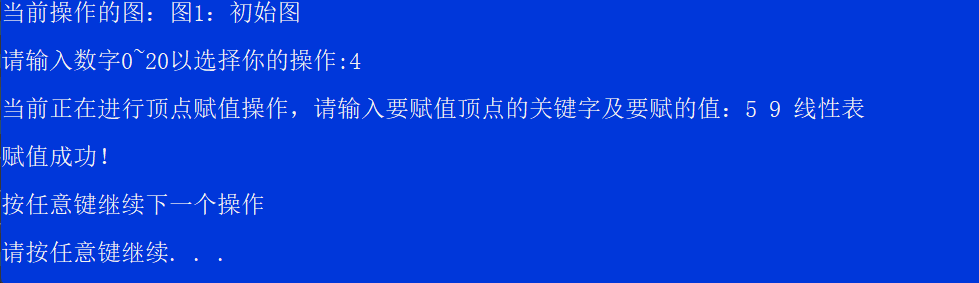
\includegraphics[scale=0.6]{./images/图/1-4.png}
			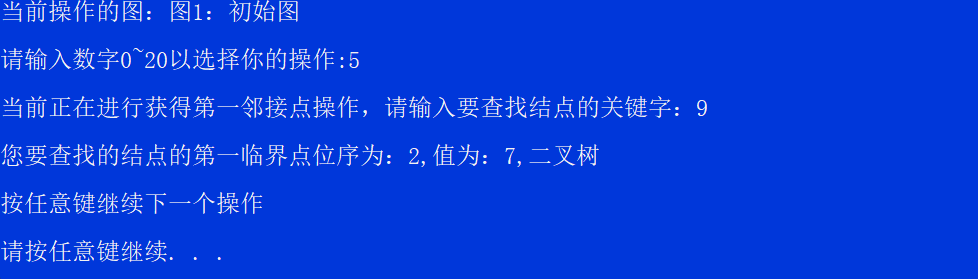
\includegraphics[scale=0.6]{./images/图/1-5.png}
			\includegraphics[scale=0.6]{./images/图/1-6.png}
			\caption{查找顶点、顶点赋值、获取邻接点测试组的截图}
			\label{fig2-7}
		\end{center}
	\end{figure}

	除标准数据外,下面测试了一些不合法数据、临界数据,依次为查找结点不存在、赋值结点不存在、获取第一邻接点时图为空、没有下一邻接点的情况,测试结果如下图\ref{fig2-8}所示。
	\begin{figure}[htb] % here top bottom
		\begin{center}
			\includegraphics[scale=0.6]{./images/图/1-1-3.png}
			\includegraphics[scale=0.6]{./images/图/1-1-4.png}
			\includegraphics[scale=0.6]{./images/图/1-1-5.png}
			\includegraphics[scale=0.6]{./images/图/1-1-6.png}
			\caption{不合法数据、临界数据测试组的截图}
			\label{fig2-8}
		\end{center}
	\end{figure}

	\newpage

	\item 插入、删除的测试
	
	对Graph1进行操作,先插入关键字为9的结点,再插入关联关键字为5和9的弧,利用深度优先搜索遍历检验正确性。再删除关键字为5的结点,删除关联关键字为7和8的弧,用广度优先搜素遍历检验正确性。测试数据如表\ref{table5}所示。
	\begin{table}
		\begin{center}
		\setlength{\tabcolsep}{2.0mm}
		\caption{插入、删除测试表}
		\label{table5}
			\begin{tabular}{c|c|c|c}
			\hline
			测试用例    			     & 输入               & 理论结果         & 测试结果\\
			\hline
			\hline			
			\multirow{6}{*}{Graph1}   	& 7 9 有向图          & 插入成功!      & 插入成功!\\
										& 8 5 9		         & 插入成功!      & 插入成功!\\
										& 11		         & 5 9 7 8 6	  & 5 9 7 8 6\\
										& 9 5			     & 删除成功! 	   & 删除成功!\\
										& 10 7 8		     & 删除成功! 	   & 删除成功!\\
										& 12			     & 8 7 6 9  	  & 8 7 6 9\\
			\hline
			\end{tabular}
		\end{center}
	\end{table}
	
	测试结果如下图\ref{fig2-9}、图\ref{fig2-10}所示。
	\begin{figure}[htb] % here top bottom
		\begin{center}
			\includegraphics[scale=0.6]{./images/图/2-7.png}
			\includegraphics[scale=0.6]{./images/图/2-8.png}
			\includegraphics[scale=0.6]{./images/图/2-11.png}
			\caption{插入、删除测试组的截图(1)}
			\label{fig2-9}
		\end{center}
	\end{figure}
	\begin{figure}[htb] % here top bottom
		\begin{center}
			\includegraphics[scale=0.6]{./images/图/2-9.png}
			\includegraphics[scale=0.6]{./images/图/2-10.png}
			\includegraphics[scale=0.6]{./images/图/2-12.png}
			\caption{插入、删除测试组的截图(2)}
			\label{fig2-10}
		\end{center}
	\end{figure}
	
	\newpage

	除标准数据外,下面测试了一些不合法数据、临界数据,依次为插入结点关键字重复、插入弧已存在、删除节点不存在、删除弧不存在的情况。测试结果如下图\ref{fig2-11}、图\ref{fig2-12}所示。
	\begin{figure}[htb] % here top bottom
		\begin{center}
			\includegraphics[scale=0.6]{./images/图/2-2-7.png}
			\includegraphics[scale=0.6]{./images/图/2-2-8.png}
			\caption{不合法数据、临界数据测试组的截图(1)}
			\label{fig2-11}
		\end{center}
	\end{figure}
	\begin{figure}[htb] % here top bottom
		\begin{center}
			\includegraphics[scale=0.6]{./images/图/2-2-9.png}
			\includegraphics[scale=0.6]{./images/图/2-2-10.png}
			\caption{不合法数据、临界数据测试组的截图(2)}
			\label{fig2-12}
		\end{center}
	\end{figure}

	\newpage

	\item 附加功能的测试

	对Graph2进行操作,求与关键字为2的结点距离小于3的所有结点,计算关键字为2和7的结点之间的最短路径,删除关键字为5的结点后,求图的连通分量。测试数据如表\ref{table6}表示。
	\begin{table}
		\begin{center}
		\setlength{\tabcolsep}{2.0mm}
		\caption{附加功能测试表}
		\label{table6}
			\begin{tabular}{c|c|c|c}
			\hline
			测试用例    			     & 输入               & 理论结果         & 测试结果\\
			\hline
			\hline			
			\multirow{3}{*}{Graph1}   	& 15 2 3             & 3 c 6 f 1 a    & 3 c 6 f 1 a\\
										& 16 2 7		     & 3		      & 3\\
										& 17		         & 2			  & 2\\
			\hline
			\end{tabular}
		\end{center}
	\end{table}

	测试结果如下图\ref{fig2-13}所示。
	\begin{figure}[htb] % here top bottom
		\begin{center}
			\includegraphics[scale=0.6]{./images/图/3-15.png}
			\includegraphics[scale=0.6]{./images/图/3-16.png}
			\includegraphics[scale=0.6]{./images/图/3-17.png}
			\caption{附加功能测试组的截图}
			\label{fig2-13}
		\end{center}
	\end{figure}


\end{enumerate}

\newpage

\subsection{实验小结}

本次实验以实现图这一数据结构及相关功能为主要目的。本章实验的难度应当是所有章节中最难的,耗时也是最长。本章的基础功能较为困难,插入和删除结点和弧实现较为复杂,而附加功能中文件和多图系统可参照前三次实验,最短路径等功能算法也较为经典,难度不大。

这次试验中我也学到了很多。深度优先搜索和广度优先搜素是在算法竞赛中甚至工程上常用的遍历算法,本次实验中多次运用了这两种算法,提高了熟练度。此外,深度优先搜索帮助我更好地理解递归的思想,广度优先搜素则让我更熟练地运用队列这一数据结构。附加功能中的最短路径问题则帮助我巩固了图论的相关知识。

本次实验中也有些地方由于掌握生疏而出现了错误。在进行删除、销毁操作时,我常常不清楚哪些结点空间应当被释放,从哪里入手,导致空间释放不正确,百思不得其解,也耗费了很多时间。这实际上是概念掌握不熟练导致的。在回顾课本、询问同学之后,最终还是正确地释放了结点空间,从错误中学到了知识。

\newpage

\section{课程的收获和建议}

% 描述通过学习该专题,有何收获,有何建议,如某专题可适当减少讲授时间、某专题可适当增加讲授内容和时间等。描述通过学习该专题,有何收获,有何建议,如某专题可适当减少讲授时间、某专题可适当增加讲授内容和时间等。描述通过学习该专题,有何收获,有何建议,如某专题可适当减少讲授时间、某专题可适当增加讲授内容和时间等。描述通过学习该专题,有何收获,有何建议,如某专题可适当减少讲授时间、某专题可适当增加讲授内容和时间等。

本次数据结构实验课程中我学到了很多,也突破了自我。这是我第一次写下超过千行的代码文件,第一次构建一个可供他人使用的“系统”,也是第一次用LaTex写下程序设计相关的实验报告。感谢一直以来辅导以及检查我的系统的老师,也感谢一直努力的自己。

关于课程整体建议提前1-2周开课,并且课程中间可以间隔一周,这样可以有更充足的时间来编写代码。

\subsection{基于顺序存储结构的线性表实现}

% 描述通过学习计算机基础知识专题,有何收获,有何建议,如某专题可适当减少讲授时间、某专题可适当增加讲授内容和时间等。描述网页的设计和实现过程中遇到的问题及如何解决。描述网页的设计和实现过程中遇到的问题及如何解决。描述网页的设计和实现过程中遇到的问题及如何解决。描述网页的设计和实现过程中遇到的问题及如何解决。描述网页的设计和实现过程中遇到的问题及如何解决。描述网页的设计和实现过程中遇到的问题及如何解决。描述网页的设计和实现过程中遇到的问题及如何解决。描述网页的设计和实现过程中遇到的问题及如何解决。

顺序表是课程中最为简单的一章。顺序存储结构使用数组实现,可以进行随机存取,也方便实现排序等功能,较为简便。本次实验最大的收获则是初步练习如何将已经编写好的函数整合到一个代码文件中,也复习了文件存取和结构体的知识。

\subsection{基于链式存储结构的线性表实现}

% 描述通过学习文档撰写工具LaTeX专题,有何收获,有何建议,如某专题可适当减少讲授时间、某专题可适当增加讲授内容和时间等。描述通过学习文档撰写工具LaTeX专题,有何收获,有何建议,如某专题可适当减少讲授时间、某专题可适当增加讲授内容和时间等。

链式存储结构线性表与上一章顺序表差别不大,基础功能只是将数组实现改为链表实现。通过本章以及与上一章的比较可以发现,算法并不因数据结构的实现方式而改变,例如对于单链表,冒泡排序、选择排序等排序算法依然成立,且实现方法相似。

\subsection{基于二叉链表的二叉树实现}

% 描述通过学习编程工具Python专题,有何收获,有何建议,如某专题可适当减少讲授时间、某专题可适当增加讲授内容和时间等。描述通过学习编程工具Python专题,有何收获,有何建议,如某专题可适当减少讲授时间、某专题可适当增加讲授内容和时间等。

二叉树是《数据结构》课程中极为重要的一章。本章中四种遍历方式都运用了递归的思想,中序遍历非递归的实现也帮助我巩固了堆栈这一数据结构的用法。附加功能中最近公共祖先、翻转二叉树等功能再次体现了递归的思想。本章结点空间的释放是实现过程中最常犯的错误,有时删除节点后再添加会导致运行错误,这就是未处理好空间分配的问题。由于在程序设计竞赛中使用数组实现二叉树较为方便,建议本章允许学生在数组和单链表中任选其一实现二叉树即可。

\subsection{基于邻接表的图实现}

% 描述通过学习计算机基础知识专题,有何收获,有何建议,如某专题可适当减少讲授时间、某专题可适当增加讲授内容和时间等。描述通过学习计算机基础知识专题,有何收获,有何建议,如某专题可适当减少讲授时间、某专题可适当增加讲授内容和时间等。

基于邻接表的图是课程最为复杂的一章,用到了先前练习的顺序表和链表。邻接表的实现方式也给最短路径等算法的实现带来了挑战。本章中关于深度优先搜索和广度优先搜素两种遍历方法的实现对我有较大的帮助,深入理解了递归思想和队列的使用。

\nocite{*} %% 作用是不对文献进行引用,但可以生成文献列表

\bibliographystyle{Experimental_Report}
\bibliography{Experimental_Report}
\setcounter{secnumdepth}{0}
\appendix

\section{附录A 基于顺序存储结构线性表实现的源程序}
\lstinputlisting[language={[ANSI]C++}]{./顺序表.cpp}
\newpage
\section{附录B 基于邻接表图实现的源程序}
\lstinputlisting[language={[ANSI]C++}]{./图.cpp}
\end{document}